\documentclass[11pt]{amsart}
\usepackage{amssymb, amstext, amscd, amsmath, amssymb}
\usepackage{mathtools, paralist, color, dsfont, rotating}
\usepackage{verbatim}
\usepackage{enumerate,enumitem}
\usepackage{tikz-cd}
%\usepackage{fullpage} 
\usepackage{float}
\usepackage{setspace}
\usepackage{todonotes}
\usepackage{algorithm}
\usepackage{algorithmic}

% change font style
%\usepackage{palatino}
%\usepackage{times}
%\usepackage{tgbonum}
%\usepackage{charter}
%\usepackage{times}

% check if all items are cited
%\usepackage{refcheck}
%%%%%

%\usepackage[notcite,notref]{showkeys}
%\usepackage{showlabels}
%\usepackage{color}
\usepackage{hyperref}
%\usepackage{tikz-cd}
\usepackage{tikz}
\usepackage{mathdots}

% boxed figures
\floatstyle{boxed}
\restylefloat{figure}

% style of text
\numberwithin{equation}{section}
%\setlength{\parskip}{1.05pt}
\footskip=20pt %for numbering of pages

\usepackage[a4paper]{geometry}
\geometry{
    tmargin= 3cm, %3cm, %1.3in, %3.5cm, %2.65cm,
    bmargin= 2.5cm, %2.3cm, %1.1in, %3cm, %2.5cm,
    rmargin= 2.5cm, %2.3cm, %1.1in, %2.75cm, %2.3cm,
    lmargin= 2.5cm %2.3cm %1.1in %2.75cm, %2.3cm
}

% quoting: if quoting package is not applicable, mute the following orders and substitute quoting <----> quote
\usepackage{quoting}
\quotingsetup{vskip=.1in}
\quotingsetup{leftmargin=.17in}
\quotingsetup{rightmargin=.17in}
%%%%%

% adjust spaces in bibliography
\let\OLDthebibliography\thebibliography\renewcommand\thebibliography[1]{
    \OLDthebibliography{#1}
    \setlength{\parskip}{0pt}
    \setlength{\itemsep}{2pt plus 0.5ex}
}

%%%%%%%%%% begin macros %%%%%%%%%%%%%%%
%
%      Cites in bold rather than roman.
\makeatletter
\def\@cite#1#2{{\m@th\upshape\bfseries%
            [{#1\if@tempswa{\m@th\upshape\mdseries, #2}\fi}]}}
\makeatother
%
% Proclamation definitions in the most emphatic (plain) style:
\theoremstyle{plain}
\newtheorem{theorem}{Theorem}[section]
\newtheorem{corollary}[theorem]{Corollary}
\newtheorem{proposition}[theorem]{Proposition}
\newtheorem{lemma}[theorem]{Lemma}
% Proclamation definitions in the less emphatic (definition) style:
\theoremstyle{definition}
\newtheorem{definition}[theorem]{Definition}
\newtheorem{example}[theorem]{Example}
\newtheorem{examples}[theorem]{Examples}
\newtheorem{counterexample}[theorem]{Counterexample}
\newtheorem{remark}[theorem]{Remark}
\newtheorem{application}[theorem]{Application}
\newtheorem{conjecture}[theorem]{Conjecture}
\newtheorem{question}[theorem]{Question}
\newtheorem*{acknow}{Acknowledgements}
\newtheorem*{details}{Details}
% Proclamation definitions in the least emphatic (remark) style:
\theoremstyle{remark}
%\newtheorem{remark}{Remark}
\newtheorem*{notation}{Notation}

%      Proof environment
\renewcommand{\proofname}{\em\textbf{Proof.}\/}
\renewcommand{\qedsymbol}{{\vrule height5pt width5pt depth1pt}}
% Change first-level `enumerate' numbering from arabic to roman.
%
\renewcommand{\labelenumi}{\textup{(\roman{enumi})} }
% properly align :=
\mathtoolsset{centercolon}
%
% Blackboard bold letters
\newcommand{\bbA}{{\mathbb{A}}}
\newcommand{\bbB}{{\mathbb{B}}}
\newcommand{\bbC}{{\mathbb{C}}}
\newcommand{\bbD}{{\mathbb{D}}}
\newcommand{\bbI}{{\mathbb{I}}}
\newcommand{\bbF}{{\mathbb{F}}}
\newcommand{\bbK}{{\mathbb{K}}}
\newcommand{\bbN}{{\mathbb{N}}}
\newcommand{\bbQ}{{\mathbb{Q}}}
\newcommand{\bbR}{{\mathbb{R}}}
\newcommand{\bbT}{{\mathbb{T}}}
\newcommand{\bbZ}{{\mathbb{Z}}}
% Capital script letters
\newcommand{\A}{{\mathcal{A}}}
\newcommand{\B}{{\mathcal{B}}}
\newcommand{\C}{{\mathcal{C}}}
\newcommand{\D}{{\mathcal{D}}}
\newcommand{\E}{{\mathcal{E}}}
\newcommand{\F}{{\mathcal{F}}}
\newcommand{\G}{{\mathcal{G}}}
\renewcommand{\H}{{\mathcal{H}}}
\newcommand{\I}{{\mathcal{I}}}
\newcommand{\J}{{\mathcal{J}}}
\newcommand{\K}{{\mathcal{K}}}
\renewcommand{\L}{{\mathcal{L}}}
\newcommand{\M}{{\mathcal{M}}}
\newcommand{\N}{{\mathcal{N}}}
\renewcommand{\O}{{\mathcal{O}}}
\renewcommand{\P}{{\mathcal{P}}}
\newcommand{\Q}{{\mathcal{Q}}}
\newcommand{\R}{{\mathcal{R}}}
\renewcommand{\S}{{\mathcal{S}}}
\newcommand{\T}{{\mathcal{T}}}
\newcommand{\U}{{\mathcal{U}}}
\newcommand{\V}{{\mathcal{V}}}
\newcommand{\W}{{\mathcal{W}}}
\newcommand{\X}{{\mathcal{X}}}
\newcommand{\Y}{{\mathcal{Y}}}
\newcommand{\Z}{{\mathcal{Z}}}
% Fraktur letters
\newcommand{\germA}{{\mathfrak{A}}}
\newcommand{\germB}{{\mathfrak{B}}}
\newcommand{\fA}{{\mathfrak{A}}}
\newcommand{\fB}{{\mathfrak{B}}}
\newcommand{\fC}{{\mathfrak{C}}}
\newcommand{\fD}{{\mathfrak{D}}}
\newcommand{\fH}{{\mathfrak{H}}}
\newcommand{\fG}{{\mathfrak{G}}}
\newcommand{\fI}{{\mathfrak{I}}}
\newcommand{\fJ}{{\mathfrak{J}}}
\newcommand{\fK}{{\mathfrak{K}}}
\newcommand{\fL}{{\mathfrak{L}}}
\newcommand{\fM}{{\mathfrak{M}}}
\newcommand{\fR}{{\mathfrak{R}}}
\newcommand{\fS}{{\mathfrak{S}}}
\newcommand{\fT}{{\mathfrak{T}}}
\newcommand{\fU}{{\mathfrak{U}}}
\newcommand{\fV}{{\mathfrak{V}}}
% Math boldface
\newcommand{\ba}{{\mathbf{a}}}
\newcommand{\be}{{\mathbf{e}}}
\newcommand{\bk}{{\mathbf{k}}}
%%%%%%%%%% end macros %%%%%%%%%%
\begin{document}
%%%%%%%%%%%%%%%%%%%%%%%%%%%%%%%%%%%%%%
\title{Matrix triangle inequality computational probabilities}


\author{Osman Jime}
\author{Jordan Kaseram}
\address{Department of Mathematics and Statistics
  \\MacEwan University \\ Edmonton, AB \\Canada}
\email{jimeo@mymacewan.ca}
\email{kaseramj@mymacewan.ca}

%%%%%%%%%%%%%%%%
\begin{abstract}
  %-Add abstract last
  The triangle inequality is a fundamental principle in mathematics and its validity is not always guaranteed in matrix theory, specifically, when dealing with the matrix absolute value.
  We investigate the how often the matrix absolute value satisfies the triangle inequality for different spaces of matrices.
  Using numerical analysis, we quantify the frequency with which the triangle inequality holds and identify key factors contributing to its success or failure.
\end{abstract}
%%%%%%%%%%%%%%%%

%\thanks{2020 {\it  Mathematics Subject Classification.} }
%\thanks{{\it Key words and phrases:} } 


\maketitle

\section{Introduction}
In this paper the field, \(\mathbb{F}\), will be used to denote the real field, \(\mathbb{R}\), and the complex field, \(\mathbb{C}\).
The triangle inequality is a fundamental concept which provides crucial relationships between distances for various structures within mathematics. 
The triangle inequality states that for any triangle, the sum of the lengths of any two sides must be greater than or equal to the length of the remaining side. 
Formally, one can state:
\[
d(A, C) \leq d(A, B) + d(B, C).
\]
\begin{example}
    Consider the following triangle:
    \begin{center}
       \begin{tikzpicture}
        % Draw the triangle
        \draw[thick] (0, 0) -- (3, 0) -- (3, 4) -- cycle;
        % Label the sides
        \node at (1.5, -0.3) {3};
        \node at (3.3, 2) {4};
        \node at (1.5, 2.3) {5};
        % Label the angles
        \node at (-0.3, 0) {$A$};
        \node at (3, -0.3) {$B$};
        \node at (3.3, 4) {$C$};
    \end{tikzpicture} 
\end{center}
 Clearly, 
$
5 \leq 3 + 4 = 7,
$
indicating the triangle inequality holds true for this example.
\end{example}

When this relationship is generalized to the real number line or complex plane, the magnitude from any number to zero results in the absolute value or modulus, respectively.
Therefore, the triangle inequality can be rewritten as follows for any $a,b \in \mathbb{F}$:
%%Maybe state the other conditions that triangle inequality have to satisfy here,
\[|a + b| \leq |a| + |b|
\]
This inequality, which always holds true in this particular field, extends naturally to matrices. The absolute value (or modulus) of a matrix  $A$ , 
denoted as  $|A| = \sqrt{A^*A}$ , is defined for any $ A \in \mathbb{M}_n(\mathbb{F})$. Given this definition, one might reasonably conjecture that
\[
|A + B| \leq |A| + |B|
\]
would similarly hold for matrices  \(A, B \in \mathbb{M}_n(\mathbb{F}).\) However, this is not always the case, and the triangle inequality can indeed fail for matrices, as noted by \cite{BK} and others.
Understanding the rate and conditions under which the triangle inequality is valid is crucial, as it have significant implications for the analysis of boundedness and convergence properties in matrix theory. 
\par This paper seeks to explore and quantify the likelihood of these failures, thereby providing deeper insights into the structural behavior of the effects of matrix absolute value on the triangle
inequality. 
Thorough investigation into sets
\begin{itemize}
    \item \(\mathbb{M}_n\left(\mathbb{Z} \cap \left\{ (-k, \ldots, k) \;\middle|\; k \in \mathbb{Z} \right\}\right)\),
    \item \(\mathbb{M}_n\left(\mathbb{Z}[i] \cap \left\{ x + i y \;\middle|\; x, y \in (-k, \ldots, k), \; k \in \mathbb{Z} \right\}\right)\),
    \item \(\mathbb{M}_n\left(\mathbb{R} \cap \left\{ [-k, k] \;\middle|\; k \in \mathbb{R} \right\}\right)\), and
    \item \(\mathbb{M}_n\left(\mathbb{C} \cap \left\{ x + i y \;\middle|\; x, y \in [-k, k], \; k \in \mathbb{R} \right\}\right)\)
\end{itemize}
 was conducted numerically using an error tolerance of \(10^{-7} \) to determine their frequency of failure.
Restricting the entry ranges allows for more control and is insightful on the behavior on the triangle inequality on the absolute value; therefore, any further discussion on the triangle
inequality will be focused on \(\mathbb{M}_n\) unless otherwise stated.

\section{Preliminaries}
In this section, we briefly revisit the concept of absolute value, interpreting it as a measure of magnitude. We then extend these ideas to matrix spaces, exploring the resulting properties and behavior.

Absolute value, or modulus, is a fundamental concept in mathematics that quantifies the magnitude or size of a given mathematical object. When extending this concept to more complex structures such as vector and matrix spaces, the notion of magnitude is generalized through the norm function, denoted as
\[
||\cdot||: \mathbb{M}_n \rightarrow \mathbb{R}.
\]
The norm function shares several key properties with the absolute value, ensuring that the concept of magnitude remains consistent and meaningful. For any matrices \(A, B, C \in S\) and a scalar \(a \in \mathbb{C}\), the norm function satisfies the following properties:
\begin{enumerate}
    \item $\|A\| \geq 0$ \text{ (Non-negative)}
    \item $ \|A\|= 0 \Leftrightarrow A = \textbf{0}_S$ \text{(Positive-definiteness)}
    \item  $\|aA\| = |a|\|A\|$ \text{(Scalar multiplication)}
    \item $\|A+B\| \leq \|A\| + \|B\|$ \text{ (Triangle inequality)}
    \item \( \|AB\| \leq \|A\|\|B\| \) \text{ (Submultiplicative)}
\end{enumerate}
These properties are crucial as they provide a consistent framework for quantifying magnitude within matrix spaces. One significant application of matrix norms is in calculating the condition number, which measures the sensitivity of a solution to perturbations. Ensuring that these properties hold is essential for the concept of magnitude to retain its practical relevance and mathematical rigor.
\par To deepen our understanding of the matrix absolute value, it is essential to introduce some foundational terminology.
\begin{definition}
    A matrix $A \in \mathbb{M}_n(\mathbb{F})$ is \textbf{positive semidefinite} (PSD) if and only if $x^* A x \geq 0$ for all $x \in \mathbb{F}^n$.
\end{definition}
\begin{definition}
    Given matrices $A_i\in\mathbb{M}_n({\mathbb{F}})$ that are PSD, the relation \(\leq\) establishes a \textbf{partial order}. This means that certain pairs of matrices may be ordred relative to each other, though not all matrix pairs are necessarily comparable. A paritial order on matrices \(A, B, C \in \mathbb{M}_n({\mathbb{C}})\) must satisfy the following properties:
    \begin{enumerate}
        \item Reflectivity: $A \leq A$
        \item Anti-symmetric: If $ A \leq B$ and $B\leq A$ then $A=B$
        \item Transitive: If $A\leq B$ and $B \leq A$ then $A\leq C$.
    \end{enumerate}
\end{definition}
An example of non-comparable matrix pairs is given by:
$$
\begin{bmatrix}
    0 & 0\\
    0 & 0
\end{bmatrix}
\nleq
\begin{bmatrix}
    -1 & 0 \\
     0 & 1
\end{bmatrix} \text{ and }
\begin{bmatrix}
    1 & 0 \\
     0 & -1
\end{bmatrix}
\nleq
\begin{bmatrix}
    0 & 0\\
    0 & 0
\end{bmatrix}.$$
When applying the concept of absolute value to a matrix, since $\mathbb{M}_n$ is a partially ordered set, this disrupts the properties as seen for absolute value for the field, $\mathbb{F}$. 
The consequence of this means that these properties are not always satisfied for arbitrary matrices.
Since absolute value for the field \( \mathbb{F} \) can be expressed as a square root function: $|a| = \sqrt{a^2}$, and applying this concept to $A \in \mathbb{M}_n(\mathbb{F})$ we say that $|A| = \left( A^*A\right)^\frac{1}{2}.$ 
It should be noted that $A^*A$ is a symmetric, positive semidefinite matrix. This square root function of matrices can be calculated easily using the following result: 
\begin{theorem}[Horn \& Johnson \cite{Horn}]
    \label{theorem1}
    Let $A \in \mathbb{M}_2(\mathbb{F})$ be Hermitian, positive semidefinite and nonzero. Let 
        $$
        \tau = \left( tr(A) + 2\sqrt{det(A)} \right)^{\frac{1}{2}}
        $$
            Then the square root of a matrix is the following:
        $$
        A^\frac{1}{2} =\tau^{-1}(A + \sqrt{det(A)}I_2),
        $$
\end{theorem}
though originally unattributed, it is stated as exercise $7.3.P26$.
\begin{proof}
    Let $A =
    \begin{bmatrix}
        a & b \\
        c & d
    \end{bmatrix}$
    be Hermitian, positive semidefinite and nonzero. Then:
    $$
    A^{\frac{1}{2}} = \frac{1}{\sqrt{ a + d + 2\sqrt{ad - bc}}}
    \begin{bmatrix}
        a + \sqrt{ad-bc} & b\\
        c & d + \sqrt{ad-bc}
    \end{bmatrix}
    $$
    Squaring this result gives the following:
    \begin{align*}
        \left(A^{\frac{1}{2}}\right)^2 &= \left(\frac{1}{\sqrt{ a + d + 2\sqrt{ad - bc}}}
    \begin{bmatrix}
        a + \sqrt{ad-bc} & b\\
        c & d + \sqrt{ad-bc}
    \end{bmatrix} \right)^2\\
    &=
    \frac{1}{ a + d + 2\sqrt{ad - bc} }
    \begin{bmatrix}
        a + \sqrt{ad-bc} & b\\
        c & d + \sqrt{ad-bc}
    \end{bmatrix}^2\\
    &=
    \frac{1}{ a + d + 2\sqrt{ad - bc} }
    \begin{bmatrix}
        a^2 + ad +2a\sqrt{ad-bc} & ab +ba + 2b\sqrt{ad-bc} \\
        ac + cd + 2c\sqrt{ad-bc} & d^2 +ad +2d\sqrt{ad-bc}
    \end{bmatrix} \\ 
    &= 
    \frac{1}{ a + d + 2\sqrt{ad - bc} }
    \begin{bmatrix}
        a(a + d +2\sqrt{ad-bc}) & b(a +d + 2\sqrt{ad-bc}) \\
        c(a + d + 2\sqrt{ad-bc}) & d(a +d +2\sqrt{ad-bc})
    \end{bmatrix} \\ 
    &= 
    \begin{bmatrix}
        a &b\\
        c & d
    \end{bmatrix}\\
    &= A.
    \end{align*}
\end{proof}
Another method to calculate the absolute value of a matrix is through the spectral decomposition algorithm. This involves applying the square root to the diagonal entries of matrix \(D\) in the decomposition, giving:
$$
|A| = \left(A^*A\right)^\frac{1}{2} = PD^\frac{1}{2}P^*.
$$
\par The properties of absolute value for $a \in \mathbb{F}$ are compared with when using $A \in \mathbb{M}_n(\mathbb{F})$.
Since $A^*A$ Hermitian and PSD, it then follows that $|A|$ is also PSD, as the square root of the diagonal entries in \(D\) remains non-negative.

\par The concept of of matrix absolute value is closely tied to the partial order defined on the space of positive semidefinite matrices. Since \(\mathbb{M}_n\) is a partially ordered set, there are instanes where matrices cannot be
directly compared using this order. This limitations can lead to the failure of certain properties typically associated with absolute value in \(\mathbb{M}_n\) when extended to matrices. Specifically, because \(\leq\) 
is a partial order, there may be matries that are not comparable, which can result in the failure of this property and others like it, hence, in general, \(|AB| \nleq |A||B|\) and \(|A+B| \nleq |A| + |B|\)
for \(A, B \in \mathbb{M}_n\). However, Mortad has shown that the equality can hold under certian conditions specifically, \(|AB| = |A||B|\), when both \(A\) and \(B\) are Hermitian, or when \(A\) and \(B\) commute provided that \(A\) is normal \cite{Mortad}.
\par When these properties, such as submultiplicativity or the triangle inequality, fail, the sense of magnitude associated with the matrix absolute value loses its reliability for tasks like analyzing convergence rates or boundedness properties. Therefore, understanding these limitations is crucial when working with matrix absolute values in more advanced mathematical contexts.

\section{Triangle Inequality Computations}
To determine if the triangle inequality has failed, one must look to determine if the difference matrix, $|A|+|B|-|A+B|$, and determine that it not positive semi-definite which is verified by its eigenvalues,
or checking the determinant of the diagonal minors. Let us first consider an example where the failure of the triangle inequality occurs.

\begin{example}
Consider: 
$$
A = \begin{bmatrix}
    -1 & 1 \\
    -1 & 1
\end{bmatrix} \quad
\text{and} \quad
I_2 = \begin{bmatrix}
    1 & 0 \\
    0 & 1
\end{bmatrix}
$$
We wish to verify that: $|A+I_2| \leq |A|+|I_2|$ is not true. It is noted that $\sqrt{I_2}=I_2$. Using Theorem \ref{theorem1} allows simple computation of the matrix absolute value for matrix $A+I_2$ and matrix $A$.
\begin{align*}
    |A+I_2| &= 
    \left|\begin{bmatrix}
        -1 & 1 \\
        -1 & 1
    \end{bmatrix} 
    +
    \begin{bmatrix}
        1 & 0 \\
        0 & 1
    \end{bmatrix}\right| 
    = 
    \left|\begin{bmatrix}
        0 & 1 \\
        -1 & 2
    \end{bmatrix}\right| \\
    &=
    \left(
    \begin{bmatrix}
        0 & -1 \\
        1 & 2
    \end{bmatrix}
    \begin{bmatrix}
       0 & 1 \\
        -1 & 2 
    \end{bmatrix}\right)^\frac{1}{2} 
    =
    \begin{bmatrix}
        1 & -2 \\
        -2 & 5
    \end{bmatrix}^\frac{1}{2}\\
    &= 
    \frac{1}{\sqrt{8}}
    \begin{bmatrix}
        2 & -2\\
        -2 & 6
    \end{bmatrix}\\
    &=
    \begin{bmatrix}
         \frac{\sqrt{2}}{2} & \frac{-\sqrt{2}}{2} \\
        \frac{-\sqrt{2}}{2} & \frac{3\sqrt{2}}{2}
    \end{bmatrix}
\end{align*}
Similarly, 
\begin{align*}
    |A| &= \left|
    \begin{bmatrix}
        -1 & 1\\
        -1 & 1
    \end{bmatrix} \right|\\
    &=
    \left(
    \begin{bmatrix}
        -1 & -1\\
        1 & 1
    \end{bmatrix}
    \begin{bmatrix}
        -1 & 1\\
        -1 & 1
    \end{bmatrix}\right)^\frac{1}{2} 
    = 
    \begin{bmatrix}
        2 & -2 \\
        -2 & 2
    \end{bmatrix}^\frac{1}{2}\\
    &= 
    \frac{1}{2}
    \begin{bmatrix}
        2 & -2\\
        -2 & 2
    \end{bmatrix}\\
    &=
    \begin{bmatrix}
        1 & -1\\
        -1 & 1
    \end{bmatrix}
\end{align*}
If we apply the triangle inequality with these three matrices found, we get the following result:
\begin{align*}
    |A+I_2| &\leq |A| +I_2 \\
    \implies\begin{bmatrix}
        \frac{\sqrt{2}}{2} & \frac{-\sqrt{2}}{2} \\
        \frac{-\sqrt{2}}{2} & \frac{3\sqrt{2}}{2}
    \end{bmatrix}
    &\leq
    \begin{bmatrix}
        1 & -1 \\
        -1 & 1
    \end{bmatrix}
    +
    \begin{bmatrix}
        1 & 0 \\
        0 & 1
    \end{bmatrix}\\
    \Leftrightarrow 
    \begin{bmatrix}
        0 & 0 \\
        0 & 0
    \end{bmatrix}
    &\leq
    \begin{bmatrix}
        2 &-1\\
        -1 & 2
    \end{bmatrix} 
    -
    \begin{bmatrix}
        \frac{\sqrt{2}}{2} & \frac{-\sqrt{2}}{2} \\
        \frac{-\sqrt{2}}{2} & \frac{3\sqrt{2}}{2}
    \end{bmatrix}\\
    \implies
    \begin{bmatrix}
        0 & 0 \\
        0 & 0
    \end{bmatrix}
    &\leq
    \begin{bmatrix}
        2 - \frac{\sqrt{2}}{2} & -1 + \frac{\sqrt{2}}{2}\\
        -1 + \frac{\sqrt{2}}{2} & 2 - \frac{3\sqrt{2}}{2}
    \end{bmatrix} 
\end{align*}
If the difference matrix $|A|+I_2-|A+I_2|$ is not positive semidefinite then the triangle inequality would have failed.
We will check the determinants of the minor diagonals for this difference matrix to determine this.
\begin{align*}
    \left|2-\frac{\sqrt{2}}{2}\right| &\approx 2 - 0.707 \\
    & = 1.23 > 0
    \text{, and}\\
    \begin{vmatrix}
         2 - \frac{\sqrt{2}}{2} & -1 + \frac{\sqrt{2}}{2}\\
        -1 + \frac{\sqrt{2}}{2} & 2 - \frac{3\sqrt{2}}{2}
    \end{vmatrix}
    &= \left( 2 - \frac{\sqrt{2}}{2}\right)\left(2 - \frac{3\sqrt{2}}{2}\right) - \left(-1 + \frac{\sqrt{2}}{2}\right)^2\\
    &= \left(4 - 3\sqrt{2} - \sqrt{2} + \frac{3}{2} - \left(1 - \sqrt{2} + \frac{1}{2}\right)\right)\\
    &= 4 - 3\sqrt{2}\\
    &\approx 4 - 4.243\\
    &= -0.234 < 0.
\end{align*}
This shows that the difference matrix is not PSD; consequently, the triangle inequality fails given the choice of $A$ and $I_2$.
\end{example}
\subsection[methods]{Computational Methods}

The Triangle Inequality of the matrix absolute value was investigated using Python. Four key tasks were implemented into their own function for this paper.

\begin{enumerate}
    \item Verifying a Triangle Inequality
    \item Computing the Matrix Absolute Value of any Matrix, $A \in M_n$
    \item Verifying the Positivity of Any Matrix, $A \in M_n$
    \item Computing a random matrix in $M_n$ of varying entry types and varying entry ranges
\end{enumerate}
The complete python project can be found in the Github repository referenced in this paper. In this appendix we provide the pseudocode for each key function, without the usage of helper functions that would be found in the full project.

\paragraph{\textbf{(i) Implementing a Test for the Triangle Inequality}} The procedure of testing the triangle inequality could have simply been included in our statistics scripts, but we wanted the flexibility of being able to test different functions as lengths, as well as changing the notion of positivity if deemed necessary.

\begin{algorithm}
    \caption{Check Triangle Inequality, \texttt{triangle\_inequality()}}
    \begin{algorithmic}[1]
        \REQUIRE{Two elements, $A$, $B$ $\in V$,}
        \REQUIRE{A function to act as length, $d: V \rightarrow W$}
        \REQUIRE{A function to act as positivity, $positive: W \rightarrow \texttt{bool}$}
        \STATE Compute lengths $d(A)$, $d(B)$, $d(A+B)$
        \STATE difference = $d(A) + d(B)-d(A+B)$
        \IF{$positive(\text{difference})==\texttt{true}$}
        \STATE \textbf{return} True
        \ELSE
        \STATE \textbf{return} False
        \ENDIF
    \end{algorithmic}
\end{algorithm}

\paragraph{\textbf{(ii) Implementing the Matrix Absolute Value}} We defined a python function for the matrix absolute value, which would serve as our length function in our triangle inequality function. The absolute value of a matrix was implemented in two ways, where the first implementation determines the square root of $A^*A$ using the Spectral Decomposition. This way is the fastest as it exploits the fact that $A^*A$ is always diagonalizable. The second implementation uses a SciPy function, \texttt{absm}, to determine the square root using the Schur Decomposition. This is the most numerically stable way of computing the square root of any matrix regardless of whether it is diagonalizable \cite{Edvin}.

\begin{algorithm}
    \caption{Compute Matrix Absolute Value (Spectral), \texttt{matrix\_absolute\_value()}}
    \begin{algorithmic}[1]
        \REQUIRE{Single matrix, $A \in M_n$,}
        \STATE{Compute $A^*A$}
        \STATE{Compute $P$, $D$ of the spectral decomposition $A^*A = PDP^*$}
        \STATE{Compute $D^\frac{1}{2}$ by taking the square root each element of $D$}
        \STATE{Compute $|A| = PD^\frac{1}{2}P^*$}
        \STATE{\textbf{return} $|A|$}
    \end{algorithmic}
\end{algorithm}

\paragraph{\textbf{(ii) Implementing a test for Matrix Positivity}} The matrix positivity was implemented in two different ways. The first implementation of determining if a matrix is positive semi-definite, solves for all the eigenvalues, and asserts than the minimum eigenvalue is greater than or equal to zero.
\begin{algorithm}
    \caption{Check Matrix Positivity (Eigenvalues), \texttt{matrix\_positivity()}}
    \begin{algorithmic}[1]
        \REQUIRE{Single matrix, $A \in M_n$,}
        \REQUIRE{Tolerance, \texttt{tol},}
        \STATE{Compute $\sigma(A)$, the set of all eigenvalues of $A$}
        \STATE{Determine $\lambda_{\min} = \min(\sigma(A))$}
        \IF{$\lambda_{\min} >$ -\texttt{tol}}
        \STATE{\textbf{return} True}
        \ELSE{}
        \STATE{\textbf{return} False}
        \ENDIF{}
    \end{algorithmic}
\end{algorithm}
The second implementation for matrices in $M_2$ asserts that the trace is greater than zero and the determinant is greater than or equal to zero, recalling that for any matrix $A$, $\text{tr} A = \sum_{i}^{n} \lambda_i$, and $\text{det} A = \prod_{i}^{n} \lambda_i$. \begin{algorithm}
    \caption{Check Matrix Positivity of $M_2$ (Trace and Determinant), \texttt{matrix\_positivity()}}
    \begin{algorithmic}[1]
        \REQUIRE{Single matrix, $A \in M_2$,}
        \REQUIRE{Tolerance, \texttt{tol},}
        \STATE{Compute $\text{tr}A = A[0,0] + A[1,1]$, the Trace of $A$}
        \STATE{Compute $\text{det}A = (A[0,0] \times A[1,1]) - (A[0,1] \times A[1,0])$, the Determinant of $A$}
        \IF{$|\text{tr}A| < \texttt{tol}$ \AND$|\text{det}A| < \texttt{tol}$}
        \STATE{\textbf{return} True}
        \ELSIF{$\text{tr}A > \texttt{tol}$ \AND$\text{det}A > \texttt{tol}$}
        \STATE{\textbf{return} True}
        \ELSE{}
        \STATE{\textbf{return} False}
        \ENDIF{}
    \end{algorithmic}
\end{algorithm}
Each implementation, requires a tolerance to determine if the minimum eigenvalue (or trace/determinant) was approximately zero. If the minimum eigenvalue is minuscule, then checking the determinant might be less likely to be near our tolerance as it is the product of all eigenvalues. If all the eigenvalues are fractional, then directly checking the minimum eigenvalue will be less likely to be near our tolerance. Alternating between different implementations of determining PSD and of the matrix absolute value were useful in demonstrating that our results were not sensitive to differences in numerical stability and reproducible through different approaches.
\subsection{Results}

The percentage of Triangle Inequality failures was investigated for matrix pairs, $A, B \in M_n$ with varying entry types and dimension. For real ($M_n(\mathbb R)$) or integer ($M_n(\mathbb Z)$) type entries, the values range from $(-k, k)$, $k\in \mathbb Z$. For Gaussian integer ($M_n(\mathbb Z[i])$) or complex ($M_n(\mathbb C)$) type entries, the values are of the form $a+bi$, where $a,b$ range from $(-k, k)$, $k\in \mathbb Z$. Sample failure percentages for each entry types were calculated from 100,000 randomly chosen pairs within a fixed entry range $(-k, k)$. True failure percentages were also calculated for pairs $A, B \in M_2(\mathbb Z)$ by exhaustively determining all possible pairs (with replacement) with entry ranges $(-k, k)$, $k \geq 7 \in \mathbb Z$. (\autoref{fig:sample_true_fail_rates_n2_varied_types_ranges})
\begin{figure}[H]
    \centering
    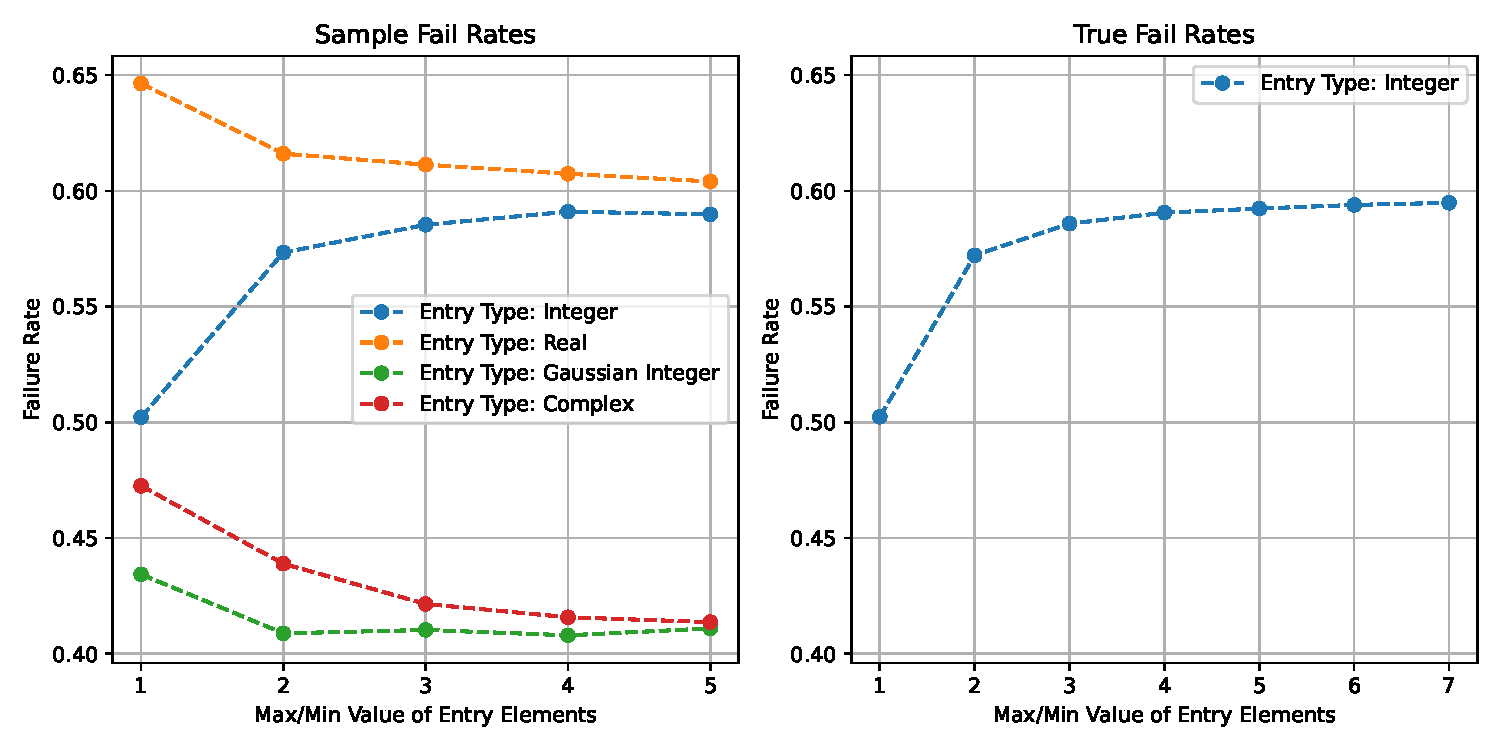
\includegraphics[width=\textwidth]{assets/sample_true_fail_rates_n2_varied_types_ranges.pdf}
    \caption{Comparison of sample and true triangle inequality failure rates of $M_2$. Each sample point contains 100,000 randomly chosen matrix pairs, with standard tolerance}\label{fig:sample_true_fail_rates_n2_varied_types_ranges}
\end{figure}

The effect of increasing the dimensions of the matrix pairs were also investigated. Sample Failure Rates for all entry types at a standard tolerance of $10^{-7}$ were produced for $2\leq n\leq 5$. (\autoref{fig:sample_fail_rate_varied_n_type_range})

\begin{figure}[H]
    \centering
    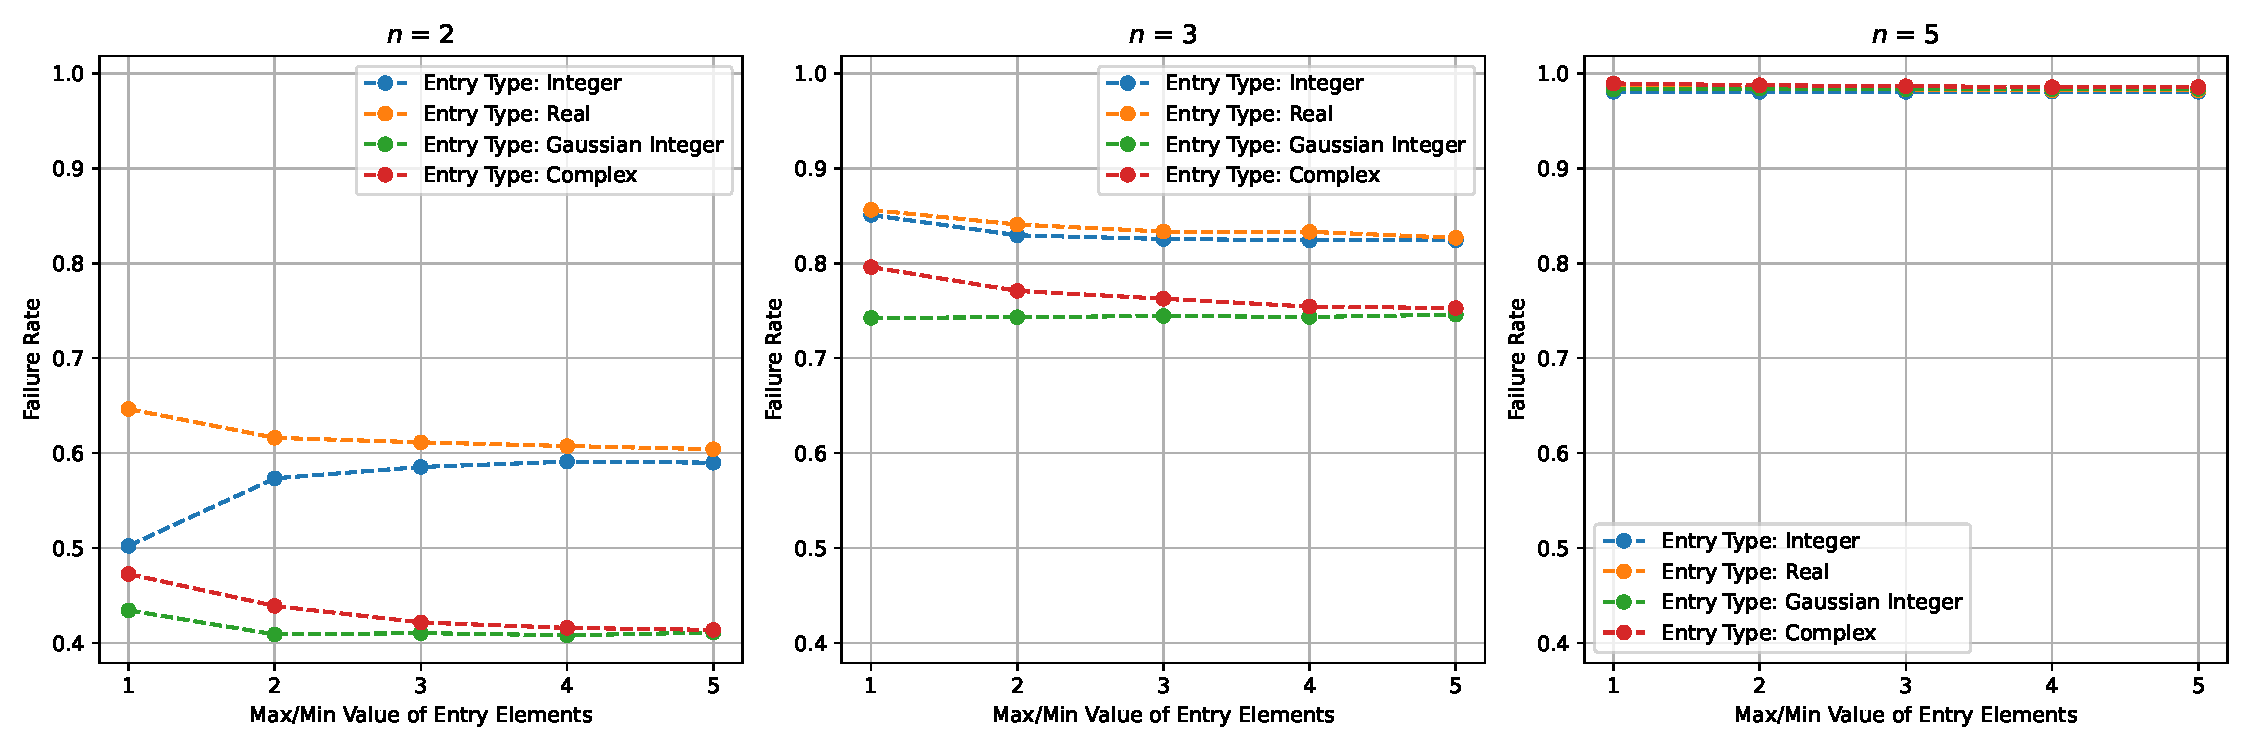
\includegraphics[width=\textwidth]{./assets/sample_fail_rate_varied_n_type_range.pdf}
    \caption{Changes in fail rate as $n$ increases. Each sample point contains 100,000 randomly chosen matrix pairs, with standard tolerance}\label{fig:sample_fail_rate_varied_n_type_range}
\end{figure}

\section{Possible Reasons for Success}
\begin{proposition}
    If \(A = B\) for \(A, B \in \mathbb{M}_n(\mathbb{F})\) then the triangle inequality will be valid.
\end{proposition}
\begin{proof}
   \begin{align*}
        |A+A| &\leq |A|+|A|\\
        \Leftrightarrow |2A| &\leq 2|A|\\
        \Leftrightarrow |2||A| &\leq 2|A|\\
        \Leftrightarrow |A| &\leq |A|.
    \end{align*} 
\end{proof}
\begin{proposition}
    If \(A\) and \(B\) are diagonal for \(A, B \in \mathbb{M}_n(\mathbb{F})\) then the triangle inequality will be valid.
\end{proposition}
\begin{proof}
    Let \(A = diag\left(a_{ii}\right)\) and \(B = diag\left(b_{ii}\right)\) for \(a_{ii}, b_{ii} \in \mathbb{F}\). Computing \(A^*A = diag\left(|a_{ii}|^2\right)\) and \(B = diag\left(|b_{ii}|^2\right)\). 
    Then \(|A| =  diag\left(|a_{ii}|\right)\) and \(|B| =  diag\left(|b_{ii}|\right)\) and the difference matrix 
    \(|A| + |B| - |A+B| = diag\left(|a_{ii}| + |b_{ii}| - |a_{ii} + b_{ii}| \right) \). Since the triangle inequality works on the modulus for \(\mathbb{F}\), then \( |a_{ii} + b_{ii}| \leq |a_{ii}| + |b_{ii}|\) is always true, hence
    all entries are non-negative, and consequently the triangle inequality for diagonal matrices will be valid.
\end{proof}
While these cases might be obvious, Mortad also discusses less obvious cases where the triangle inequality is satisfied.
\begin{theorem}[Mortad \cite{Mortad}] %its theorem 3.4 in Mortads paper
    \label{theorem2}
    Let $A, B \in \mathbb{M}_n(\mathbb{F})$ such that:
    \begin{enumerate}
        \item $AA^* = A^*A$ (Normal)
        \item $BB^* \leq B^*B$ (Hyponormal)
        \item $AB = BA$ (Commutative), 
    \end{enumerate}
    \text{ then:} $|A+B| \leq |A|+|B|$
\end{theorem}

\begin{example}
    Let \[ A = 
    \begin{bmatrix}
        -1 & 0 \\
        0 & -1
    \end{bmatrix} \text{ and }
    B = \begin{bmatrix}
        -1 & 1\\ 
        -1 & -1
    \end{bmatrix} \]
    It is clear that \(A\) and \(B\) are commutative, and \(A\) is normal. We check that \(B\) is hyponormal as follows: 
    \begin{align*}
        B^*B - BB^* &=
        \begin{bmatrix}
            -1 & -1\\ -1 & 1
        \end{bmatrix}
        \begin{bmatrix}
            -1 & 1 \\ -1 & -1
        \end{bmatrix}
        -
        \begin{bmatrix}
            -1 & 1 \\ -1 & -1
        \end{bmatrix}
        \begin{bmatrix}
            -1 & 1\\ -1 & 1
        \end{bmatrix}\\
        &=
        \begin{bmatrix}
            2 & 0 \\ 0 & 2
        \end{bmatrix}
        - 
        \begin{bmatrix}
            2 & 0 \\ 0 & 2
        \end{bmatrix}\\
        &= 0
    \end{align*}
    showing that \(B\) is normal. Therefore, by Theorem \ref{theorem2} the triangle inequality results will be valid. Verifying this claim with 
    \[
    |A| = \begin{bmatrix} 1 & 0 \\ 0 & 1 \end{bmatrix}, \quad
    |B| = \begin{bmatrix}  \sqrt{2} & 0 \\ 0 & \sqrt{2} \end{bmatrix} \text{ and }
    |A+B| = \begin{bmatrix} \sqrt{5} & 0 \\ 0 & \sqrt{5}   \end{bmatrix}
    \]
    produces the difference matrix
\begin{align*}
    |A|+|B|-|A+B| &= 
    \begin{bmatrix} 1 +  \sqrt{2} - \sqrt{5} & 0 \\ 0 &  1 +  \sqrt{2} - \sqrt{5} \end{bmatrix} \\
    &\approx
    \begin{bmatrix}
        0.178 & 0 \\ 0 & 0.178
    \end{bmatrix}\\
    &\geq
    0.
\end{align*}
\end{example}

While these matrix pairs will always satisfy the triangle inequality, they make up a small fraction of the of the total pairs that pass. The exhaustive search method for matrices in
$
\mathbb{M}_2
$
with integer entries between $-1$ and $1$ resulted with finding $337$ pairs which satisfy these conditions out of a total of $3265$ pairs passed; therefore, these pairs make up approximately $10.3\%$ of these successes.
When the range value is increased to be between $-2$ and $2$, $3345$ of these pairs were found; however, the frequency of these pairs dropped to $2\%$.
Increasing the integer range further dramatically drops this frequency of these to be less than $1\%$.

The random search method mirrors these results for integers between the same range values when using a sample size of $100,000$ random matrix pairs. 
When using this search method with complex integer entries between \(-1\) and \(1\) there are approximately $0.24\%$ matrix pairs successes found and this became $0\%$ as the entry range increased further.
This does not mean these pairs cease to exist since $\{-1,0,1\} \subseteq \{-2,-1,0,1,2\}$ and pairs were found between $-1$ to $1$ entry range, but rather implies that these pairs are very sparse.
Similarly when considering matrices with real and complex number entries these percentage of pairs was found to be $0\%$.
This does not reflect the true percentage since these pairs were already found to exist and $\mathbb{Z} \subseteq \mathbb{F}$. 
These percentages being $0$ might be an artifact by the density of the field, $\mathbb{F}$, which may not find any pairs given the how random numbers are generated in python.

\begin{figure}[H]
    \centering
    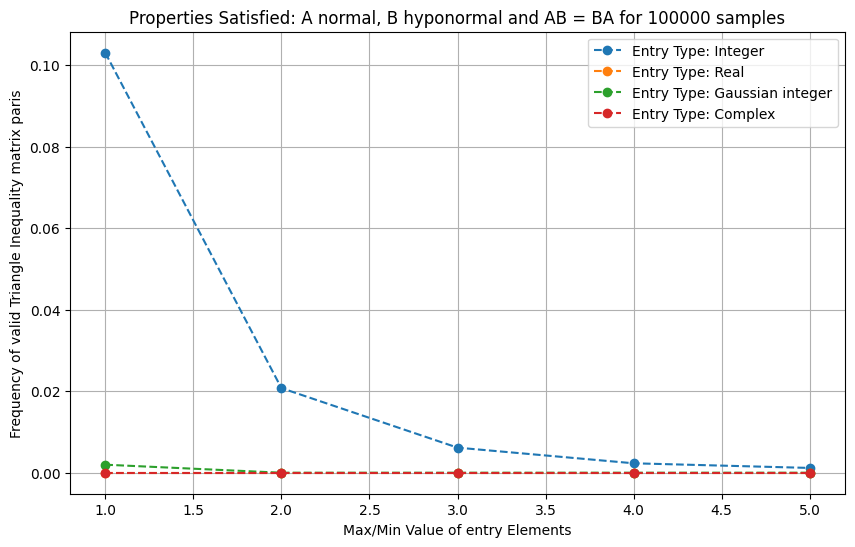
\includegraphics[scale = 0.6]{assets/theorem1plot.png}
    \caption{Random search method for matrix pairs that satisfy Theorem \ref{theorem2} for $A, B \in \mathbb{M}_2.$}
\end{figure}


\par Another case where the triangle inequality will always pass is when:
\begin{theorem}[Mortad \cite{Mortad}] %Theorem 3.15 in Mortads paper
    \label{theorem3} 
    Let $A, B \in \mathbb{M}_n(\mathbb{F})$ such that:
    \begin{enumerate}
        \item $AA^* = A^*A$ (Normal)
        \item $AB = BA$ \text{(Commutative)}
        \item $A^*B + B^*A \leq 0$,
    \end{enumerate}
     \text{ then:} $|A+B| \leq |A|+|B|$
\end{theorem}


\begin{example}[Using Theorem \ref{theorem3}]
    Consider: 
    $$
    A = \begin{bmatrix}
        -1 & 0 \\ 0 & -1
    \end{bmatrix} \quad
    \text{and} \quad
    B = \begin{bmatrix}
        0 & -1 \\ 1 & 1
    \end{bmatrix}
    $$
    Clearly $A$ and $B$ commute, and checking the inequality results in:
    \begin{align*}
        A^*B + B^*A &=
        \begin{bmatrix}
            -1 & 0 \\ 0 & -1
        \end{bmatrix}
        \begin{bmatrix}
            0 & -1 \\ 1 & 1
        \end{bmatrix} + 
        \begin{bmatrix}
            0 & 1 \\ -1 & 1
        \end{bmatrix}
        \begin{bmatrix}
            -1 & 0 \\ 0 & -1
        \end{bmatrix}\\
        &= 
        \begin{bmatrix}
            0 & 1 \\ -1 & -1
        \end{bmatrix} + 
        \begin{bmatrix}
            0 & -1 \\ 1 & -1
        \end{bmatrix}\\
        & = 
        \begin{bmatrix}
            0 & 0 \\ 0 & -2
        \end{bmatrix}\\
        &\leq
        \begin{bmatrix}
            0 & 0 \\ 0 & 0
        \end{bmatrix}
    \end{align*}
    Then the triangle inequality is guaranteed to succeed. We verify with the results with the following:
        $
        |B| = 
        \begin{bmatrix}
            \frac{2\sqrt{5}}{5} & \frac{\sqrt{5}}{5} \\
            \frac{\sqrt{5}}{5} & \frac{3\sqrt{5}}{5}
               \end{bmatrix}
        $
    and $ |A+B| = \begin{bmatrix}
        \frac{3\sqrt{5}}{5} & \frac{\sqrt{5}}{5} \\
            \frac{\sqrt{5}}{5} & \frac{2\sqrt{5}}{5}
    \end{bmatrix}$
    and with
    \begin{align*}
        |A|+|B|-|A+B| &= \begin{bmatrix} 
            1-\frac{\sqrt{5}}{5}& 0 \\ 0 & 1 + \frac{\sqrt{5}}{5}
        \end{bmatrix}\\
        &\approx
        \begin{bmatrix}
            0.553 & 0 \\ 0 & 1.447
        \end{bmatrix}\\
        &\geq
        \begin{bmatrix}
            0 & 0 \\ 0 & 0
        \end{bmatrix}.
    \end{align*}
    This shows that it passes.
\end{example}


The exhaustive search method for integer entries between $-1$ and $1$ found $377$ pairs which satisfies this new theorem resulting \(11.5\%\) of these pairs
making up the population of total successes.
When increasing the integer entry range to $-2$ and $2$ there are $4145$ matrix pairs which satisfy Theorem \ref{theorem3} resulting these pairs making up approximately $2.5\%$ of total successes.
As this entry range increases further the frequency of these matrix pairs falls below $1\%$.
Once again the random search method for integers mirrors the results of the exhaustive with a sample size of $100,000$ is used.
When the matrix is populated with complex integers there is approximately $3.3\%$ of these matrix pairs with the entry range of $-1$ to $1$.
Increasing the entry range with these matrices resulted with the frequency decreasing to less than $1\%$.
The real field and complex field both result with $0\%$ for all entry ranges tested, however as previously discussed, is likely due to an artifact. 
\begin{figure}[H]
    \centering
    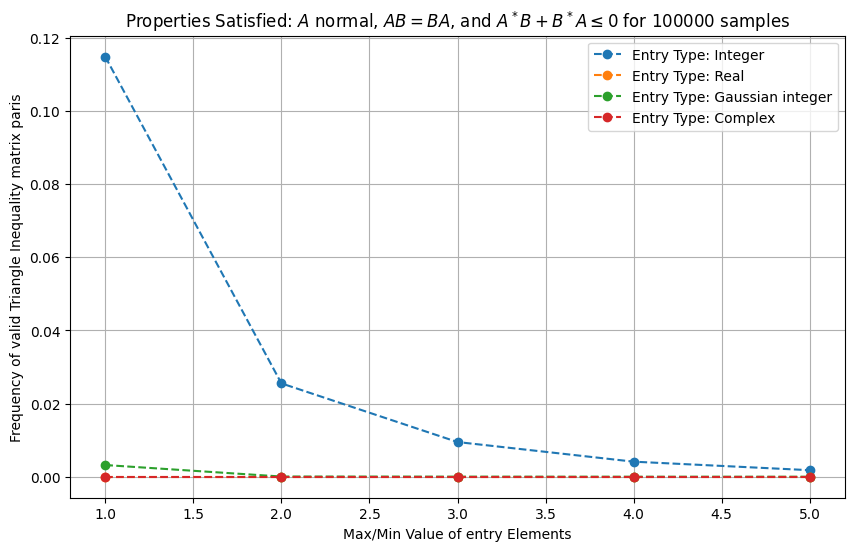
\includegraphics[scale = 0.6]{assets/theorem2plot.png}
    \caption{Random search method for matrix pairs that satisfy Theorem \ref{theorem3} for $A, B \in \mathbb{M}_2.$}
\end{figure}
\par Matrices in higher dimensions for Mortad's theorems were examined using the random search method only due to hardware limitations. The amount of matrix pairs that satisfied
these theorems was found to be negligible when compared with pairs which inherently satisfy the triangle inequality since Mortad's pairs make up less then \(1\%\) of them in \(\mathbb{M}_3\) and \(0\%\)
for \(\mathbb{M}_n\),  \(n \geq 4 \). In \(\mathbb{M}_3(\mathbb{Z} \cap \{ -1, 0, 1\} )\) the frequency for Theorem \ref{theorem2} is approximately \(0.03\%\) and for Theorem \ref{theorem3} it is
\(0.13\%\). Comparing these frequencies shows that there are more than four times the amount of pairs in Theorem \ref{theorem3} than in Theorem \ref{theorem2}. This behavior was present in \(\mathbb{M}_2\)
also and would suggest that there are more matrix pairs for Theorem \ref{theorem3} for which the triangle inequality is valid for \(\mathbb{M}_n\) than pairs found in Theorem \ref{theorem2}.

\par While Mortad's \cite{Mortad} theorems give some reasons for when the triangle inequality is valid, these pairs are very sparse in their contribution to the to set of valid matrix pairs
which satisfies the triangle inequality. 

\section*{Glossary}

% A
\begin{glossary}
    \textbf{Absolute Value (Moudlus) for \(\mathbb{F}\):} The non-negative value of a real or complex number without regard to its sign.
     For a real number \(a\), it is denoted as \(|a|\), and for a complex number \(z = a + bi\), it is \(\sqrt{a^2 + b^2}\).
\end{glossary}

\begin{glossary}
    \textbf{Absolute Value (Moudlus) for \(\mathbb{M}_n\left(\mathbb{F}\right)\):} For a matrix \(A\), the absolute value \(|A|= (A^*A)^{1/2}\), 
    where \(A^*\) is the conjugate transpose of \(A\).
\end{glossary}

% C
\begin{glossary}
    \textbf{Condition Number:} A measure of the sensitivity of a matrix’s inverse to changes or errors in the input. 
    It is defined as \(cond(A) = ||A|| \cdot ||A^{-1}|| \) or the ratio of the largest to smallest singular values.
\end{glossary}

% D
\begin{glossary}
    \textbf{Determinant:} A scalar-valued function for entries of a square matrix denoted \(det(A) \) in this paper.
\end{glossary}

% E
\begin{glossary}
    \textbf{Eigenvalue:} If \(A\) is a square matrix, then \(\lambda\) is called an eigenvalue if \(A \textbf{x} = A \lambda\) for \(\textbf{x} \in \mathbb{F}^n \setminus \{0\}\).

\end{glossary}

\begin{glossary}
    \textbf{Eigenvector:} If \(A\textbf{x} = A \lambda\) the corresponding \(\textbf{x}\) is the eigenvector of A corresponding to the eigenvalue \(\lambda\).
\end{glossary}

% F
\begin{glossary}
    \textbf{Field:} A set \(F\) which two binary operations, addition and multiplication, which satisfies the field axioms.
\end{glossary}

% H
\begin{glossary}
    \textbf{Hermitian Matrix:} A matrix which is equal to its conjugate transpose, ie \(A = A^*\).
\end{glossary}

% N
\begin{glossary}
    \textbf{Normal Matrix:} A matrix which commutes with its conjugate transpose, ie \(A^*A = AA^*\).
\end{glossary}

% P 
\begin{glossary}
    \textbf{Positive semi-definite Matrix:} Matrix \(A\) is positive semidefinite if any non-zero vector \(\textbf{x}\) 
    the product 
\(\textbf{x}^*A\textbf{x} \geq 0 \). Such matrices have non-negative eigenvalue.
\end{glossary}

% S 
\begin{glossary}
    \textbf{Schur Decomposition:} Takes an arbitrary square matrix \(A\) then it is decomposed into a unitarily simmilar matrix \(U\) and 
    an upper triangular matrix \(T\), so \(A = UTU^*\). 
\end{glossary}

\begin{glossary}
    \textbf{Spectral Decomposition:} Takes an arbitrary square matrix \(A\) and using its eigenvectors to produces a unitary matrix \(P\)
    and eigenvalues to produces diagonal matrix \(D\) so \(A = PDP^*\)
\end{glossary}

% T 
\begin{glossary}
    \textbf{Trace:} The sum of the diagonal elements in a square matrix \(A\).
\end{glossary}

\begin{thebibliography}{99}

    \bibitem{BK}
    Bhatia, F. Kittaneh, {\em The matrix arithmetic–geometric mean inequality revisited}, Linear Algebra and its Applications {\bf 428} (2008), 2177–2191.
    %People have pointed out that the triangle inequality fails.
    \bibitem{Horn}
    Horn, R. A., \& Johnson, C. R.  \textit{Matrix analysis}. Cambridge university press. (2012).

    \bibitem{Mortad}
    Mortad, M.H. On the absolute value of the product and the sum of linear operators. Rend. Circ. Mat. Palermo, II. Ser 68, 247–257 (2019).

    \bibitem{Edvin}
    Edvin Deadman, Nicholas J. Higham, Rui Ralha, Blocked Schur Algorithms for Computing the Matrix Square Root, Lecture Notes in Computer Science, 7782. pp. 171-182 (2013).

    \bibitem{GitHub}
    Jordan Kaseram, Osman Jime, Triangle Inequality Tests of Matrix Absolute Value, Version 1.0, MacEwan University, Edmonton AB Canada (2024). See http://mctdh.uni-hd.de


\end{thebibliography}

\input{src/appendix}

\end{document}

